As part of this project, an Android application will be developed for recording a smartphone's microphone audio and sending it to a central computer for further processing. The inner workings of the Android architecture are detailed in \cite{Brahler2010}, including extensive explanations of the Dalvik VM, native applications and power management. However, it was written in 2010, so some caution is advised as the Android platform has not stood still since then. Specifically, the report describes Android 2.2, whilst the most recent Android version is 5.1.1. The version on the Nexus 5 phones we will be using is 4.4.2. Since Android version 5.0, the Dalvik VM has been removed in favor of the Android Runtime (ART), promising higher performance \cite{android-art}.

The standard way to develop an application for Android is using the SDK (Software Development Kit). This allows one to write Java applications which run on the desired Android version. For tighter control over low-level functionality and potential increase performance, Android provides a NDK (Native Development Kit) which allows a user to write part of his application in a native language such as C, C++ or assembly \cite{liu2013}. The NDK is not needed for all programs, and not all programs benefit from its use. Examples where the NDK can boost performance are multimedia applications and scientific computing. The \textit{Android Native Development Cookbook} \cite{liu2013} contains information on developing native applications for Android, workspace setup instructions, gives argumentation for choosing the SDK or the NDK and has a lot of code examples. This book is definitely useful if it is decided to write a (partially) native application. Another good source of developer information is Google's developer website of the Android platform, for NDK \cite{android-ndk} and SDK \cite{android-getting-started}.

Because Android is not a real-time OS, timing issues might arise during development. Maya et al.\ \cite{Maya2010} note the lack of these capabilities and propose four different architectures for Android that would make it suitable for real-time systems. These proposed architectures include swapping out the Linux kernel for a real-time equivalent, replacing or supplementing the Dalvik VM with a real-time counterpart or adding a new hypervisor to oversee both the Android operating system in one partition and a separate real-time partition. The implementation of these real-time Android supplements is non-trivial and well beyond the scope of our thesis. Since the primary function of our application is recording sound and sending it over a (Wi-Fi) network, performance issues that can only be solved using a real-time OS are not expected.

\subsection{Clock synchronization}
\label{subsec:synch}
Separating sources in situations where only an approximation of the source signal (e.g. the recordings of the various microphones) is known is called blind source separation (BSS) \cite{wehr2004}. This problem is schematically shown in figure \ref{fig:bss}. In order to achieve this, and perform beamforming, the sampled microphone recordings must be synchronized in time and frequency.

\subsubsection{Sampling rate offset}
The offset in frequency is called sampling rate offset (SRO) \cite{wehr2004} and alternatively as clock skew \cite{Schmalenstroeer2015}. Figure \ref{fig:bss_sensitivity} shows one practical instance of the influence of SRO with respect to the gain measured when combining multiple sources. It is obvious that the offset of even a few hertz is devastating for the resulting SNR.

Cherkassky et al.\ \cite{cherkassky2014blind} propose a method to estimate, for each node (i.e. microphone), the SRO based on the cross wavelet transform (CWT) derived from correlation processing. This is proven to be optimal for signals contaminated by additive Gaussian white noise. The sampling frequency $f_s^m$ at each node (smartphone) $m$ can be expressed as $f_s^m=f_s/a_m$, where $f_s$ represents the sampling frequency at a reference node and $1/a_m$ the SRO factor. Cherkassky gives a method for estimating $1/\hat{a}_m$ based on maximizing a discrete-time version of the CWT. The SRO can then be compensated using (fourth-order) Lagrange polynomial interpolation, outlined in \cite{golan2012}.

Golan et al.\ \cite{golan2012} propose a different method for SRO estimation. This method is based on the fact that sample rate offset between microphones $s$ and $r$:
\[
f_{s,r} = (1 + \epsilon_{r}) f_{s}
\]
yields a phase shift proportional to frequency in the (discrete) Fourier domain:
\[
\theta_{s,r}^{\ell}[k] = \exp\left(j \frac{2 \pi k \ell \epsilon_{r}}{K}\right) \theta_{s,r}[k]
\]

Therefore, they estimate the SRO $\hat{\epsilon}_{n}$ by computing the phase shift for all microphones $s$, (discrete) frequencies $k$ and time segments $i$, then averaging the results.

Figure \ref{fig:sro_coherence} shows the improved coherence between two simultaneous microphone recordings on low-cost hardware after SRO correction using the CWT and Langrange polynomials method described above.

\begin{figure}[b!]
\centering
\caption{}
~
        \begin{subfigure}[b]{0.27\textwidth}
                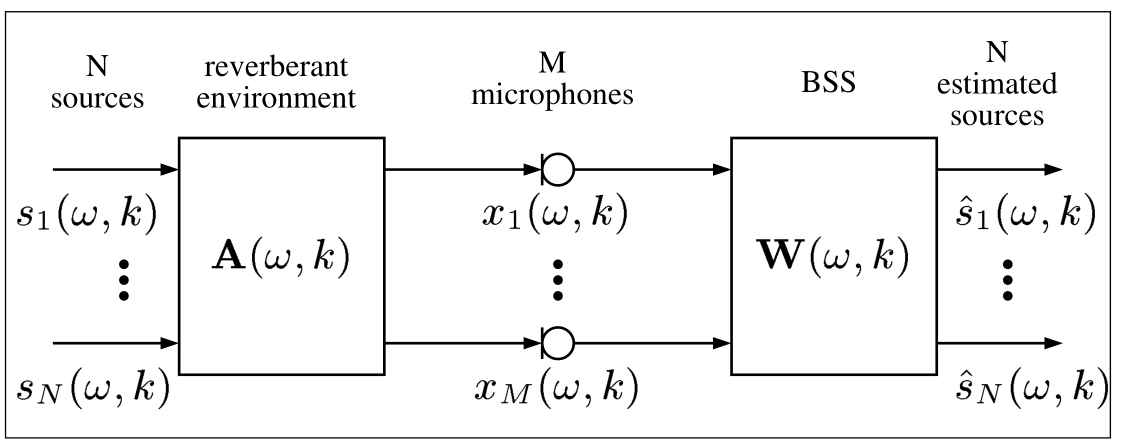
\includegraphics[width=\textwidth]{images/bss}
                \caption{Blind source separation (BSS) as schematized in \cite{wehr2004}.}
                \label{fig:bss}
        \end{subfigure}
        ~ %separation between figures
        \begin{subfigure}[b]{0.27\textwidth}
                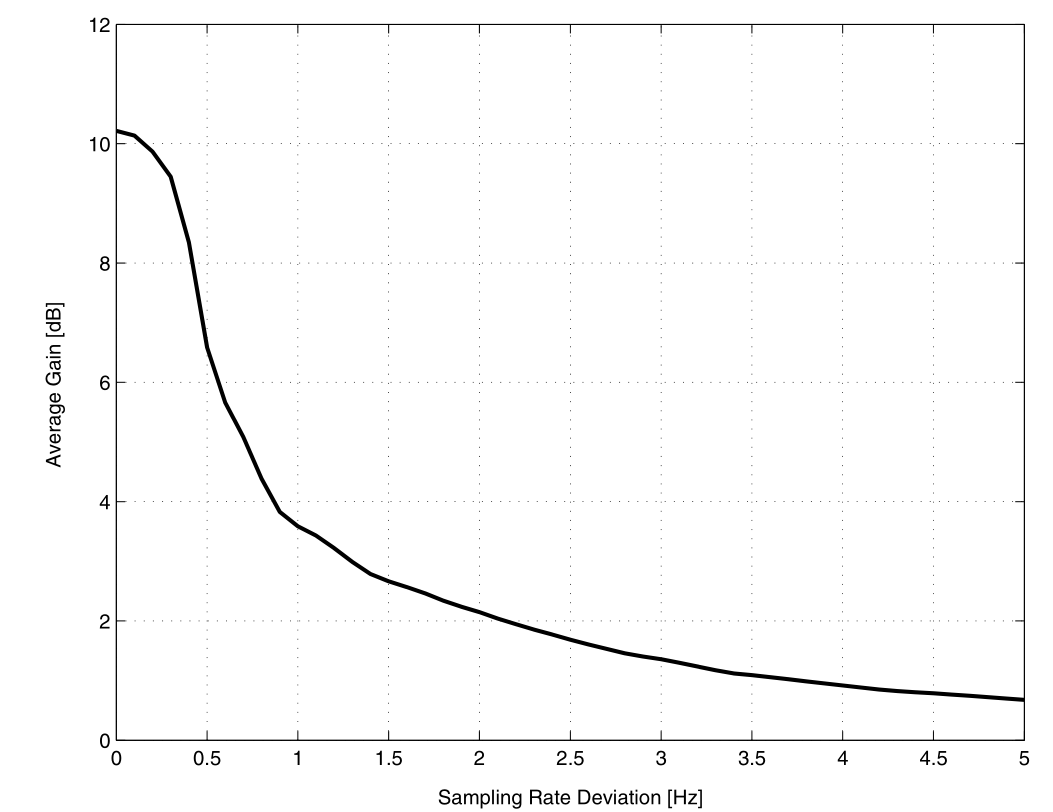
\includegraphics[width=\textwidth]{images/bss_sensitivity}
                \caption{The influence of SRO to the gain of additive signals \cite{wehr2004}.}
                \label{fig:bss_sensitivity}
        \end{subfigure}
        ~ %separation between figures
        \begin{subfigure}[b]{0.27\textwidth}
                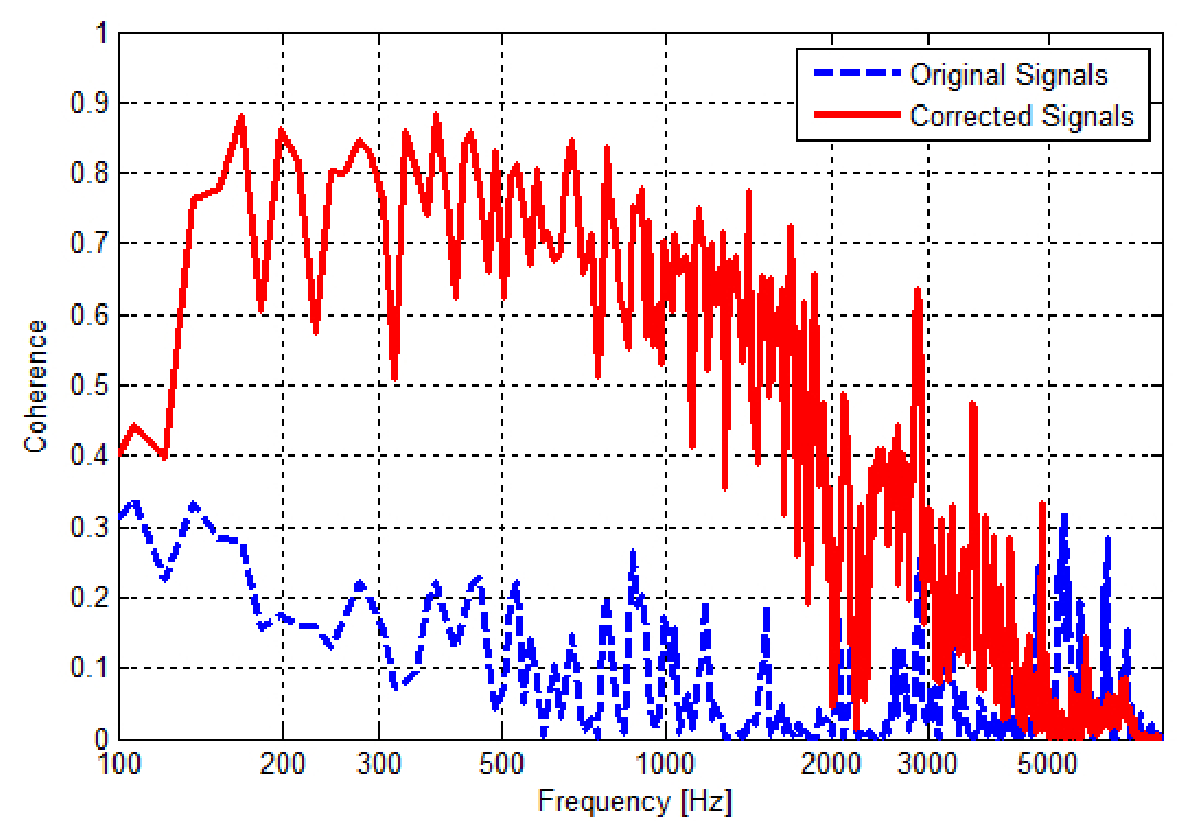
\includegraphics[width=\textwidth]{images/sro_coherence}
                \caption{SRO correction leads to improved coherence between two microphone recordings \cite{cherkassky2014blind}.}
                \label{fig:sro_coherence}
        \end{subfigure}
~
\end{figure}

A distributed SRO correction algorithm implemented in a hardware/software combination is explained in \cite{Schmalenstroeer2015}. The advantages of using their distributed method are: robustness to a failing master clock, less communication overhead and less reconfiguration when new (microphone) nodes join the network. However, to obtain these results, dedicated hardware is used which is unsuitable for our application.

\subsubsection{Time offset}
The offset in (start) time of recording must also be controlled. Several methods for this are detailed in \cite{wehr2004} and deemed unsuitable for their purposes: Network Time Protocol (NTP) which is used worldwide for clock synchronization via the Internet achieves errors in the order of tens of milliseconds. When audio is segmented into 20 millisecond blocks as with normal phone calls, this error is unacceptably high. GPS also yields timing information, and with much higher accuracy than NTP would allow: within 340 nanoseconds (95\% certainty) using a Standard Positioning Service (SPS) device. However, GPS requires line-of-sight to satellites and is not intended for indoor use, making it unsuitable for a conference room environment. The solution implemented by Wehr et al.\ \cite{wehr2004} uses a secondary channel operating at radio frequencies. Since the goal of this project is to synchronize smartphones without additional hardware, this too is unsuitable for our application.

Ballew et al.\ \cite{ballew2011} investigate time synchronization applied to concert recordings on YouTube for music enhancement purposes, but do this offline, e.g. after the complete recording has taken place. This approach is partially suited for our application in showing that offline synchronization is possible, given that the smartphones send an accurate timestamp to the central computer along with the recording. However, this does not solve the problem of labeling the signals with timestamps.

\subsection{Processing latency and speech quality}
It is also useful to evaluate the latency added by the full system as it processes the microphone signals. The \textit{International Telecommunication Union} (ITU) claims in its \textit{G.114} recommendation \cite{itu-g114} that total system delays above 400 ms are unacceptable, and delays under 150 ms are essentially transparent for voice communications. This recommendation derives from the \textit{E-model} \cite{itu-g107}, a perceptual model for the influence of various impairments on the subjective speech quality perceived by a listener. This perceived speech quality is measured using a \textit{mean opinion score}: a value on a scale of one (worst) to five (best), computed as the arithmetic average result of ratings given by individual listeners \cite{itu-p800}.

\subsection{Orientation estimation}
In order to compensate for the directivity of the smartphone microphones, their orientation must be accurately known. This can be accomplished by processing the data from sensors inside each smartphone. Android devices can have a variety of sensors, most importantly a 3D magnetometer and accelerometer \cite{android-sensors}. Orientation can be computed from these directly, and if this estimate proves to be too noisy, the data can be filtered to improve accuracy. Goslinski et al.\ \cite{goslinski2015} compare several such filter algorithms in the context of implementation on Android devices. The article links to code for the various implementations, finally concluding that use of these filters -- particularly their adaptive extended Kalman filter -- can significantly improve orientation estimate accuracy.